% SkyNYC final report. Build: tectonic skynyc-final-report.tex
\documentclass[11pt]{article}

\usepackage[margin=1.1in]{geometry}
\usepackage[T1]{fontenc}
\usepackage[utf8]{inputenc}
\usepackage{lmodern}
\usepackage{microtype}
\usepackage{graphicx}
\usepackage{booktabs}
\usepackage{array}
\usepackage{float}
\usepackage{caption}
\usepackage{xcolor}
\usepackage{titlesec}
\usepackage[hidelinks]{hyperref}
\usepackage{enumitem}

\definecolor{ink}{HTML}{1F2328}
\definecolor{muted}{HTML}{57606A}
\definecolor{rule}{HTML}{D0D7DE}

\titleformat{\section}{\Large\bfseries\color{ink}}{\thesection}{0.8em}{}
\titleformat{\subsection}{\large\bfseries\color{ink}}{\thesubsection}{0.8em}{}
\captionsetup{font={small,color=muted},labelfont=bf}
\setlist{itemsep=2pt,topsep=4pt}
\renewcommand{\arraystretch}{1.25}

\newcommand{\code}[1]{\texttt{\small #1}}

\title{\vspace{-1.2em}\textbf{SkyNYC}\\[0.35em]
\large Measuring weather impact on New York airport arrivals\\
from raw aircraft telemetry\\[0.5em]
\normalsize Final report}
\author{Gil Lu}
\date{August 2026}

\begin{document}
\maketitle

\begin{abstract}
\noindent
SkyNYC derived airport operational events --- arrivals, holding patterns, and
go-arounds --- for JFK, LaGuardia, and Newark directly from raw ADS-B position
telemetry, validated them daily against an independent arrivals record, and
joined them with official weather observations to measure how conditions
degrade arrival operations. No delay feed, arrivals feed, or event feed was
consumed at any point: every operational event was computed by per-aircraft
state machines over a Kafka-buffered position stream, and the accuracy of that
derivation was published as a daily precision/recall score rather than claimed.
Over a fifteen-day continuous run the detectors identified 26{,}303 arrivals,
scored against 28{,}331 independently recorded ones: mean daily precision
96.7\%, mean daily recall 93.0\% across the three airports. A companion historical layer
rebuilt 181~million federal on-time records (1987--2026) into a Delta Lake
medallion, quantifying the thesis at climatological scale: average arrival
delay on the worst weather days runs eight to fourteen times higher than on
clear days. Total infrastructure cost: about \$26 of compute and \$10--15 of cloud
storage and batch services.
\end{abstract}

\section{The question and the approach}

The business question: how much do arrival rates fall --- and holding and
go-arounds rise --- as conditions degrade from VFR to IFR, and which weather
variable (visibility, ceiling, wind and gusts) leads the degradation?

The engineering premise that makes the project interesting: the operational
events needed to answer it exist in no public feed. The FAA publishes delay
status, not events; airlines publish schedules, not go-arounds. SkyNYC
therefore treats event \emph{derivation} as the core deliverable --- and holds
that derivation to a published accuracy standard, scored daily against ground
truth that the detectors never see.

The system ran in two layers:

\begin{itemize}
\item \textbf{Live streaming layer} (2026-08-12 to 2026-08-26): OpenSky
Network ADS-B state vectors polled every 30\,s and NOAA/NWS observations and
alerts polled every 5/2 minutes, buffered in Kafka, processed by Spark
Structured Streaming into a bronze Parquet archive on Azure ADLS~Gen2, a
live-position serving table, and a stream of derived flight events in
Postgres. dbt built hourly marts on top; Dagster orchestrated the batch edges
(daily ground-truth pull, hourly builds, nightly backup).
\item \textbf{Historical batch layer}: 38 years of BTS on-time performance
(181M rows) and 4.3M METAR observations, landed by Azure Data Factory and
built into a bronze/silver/gold Delta medallion by Databricks jobs that
Dagster triggers over the Jobs API. Postgres remained the only serving store.
\end{itemize}

\section{Architecture}

\begin{figure}[H]
\centering
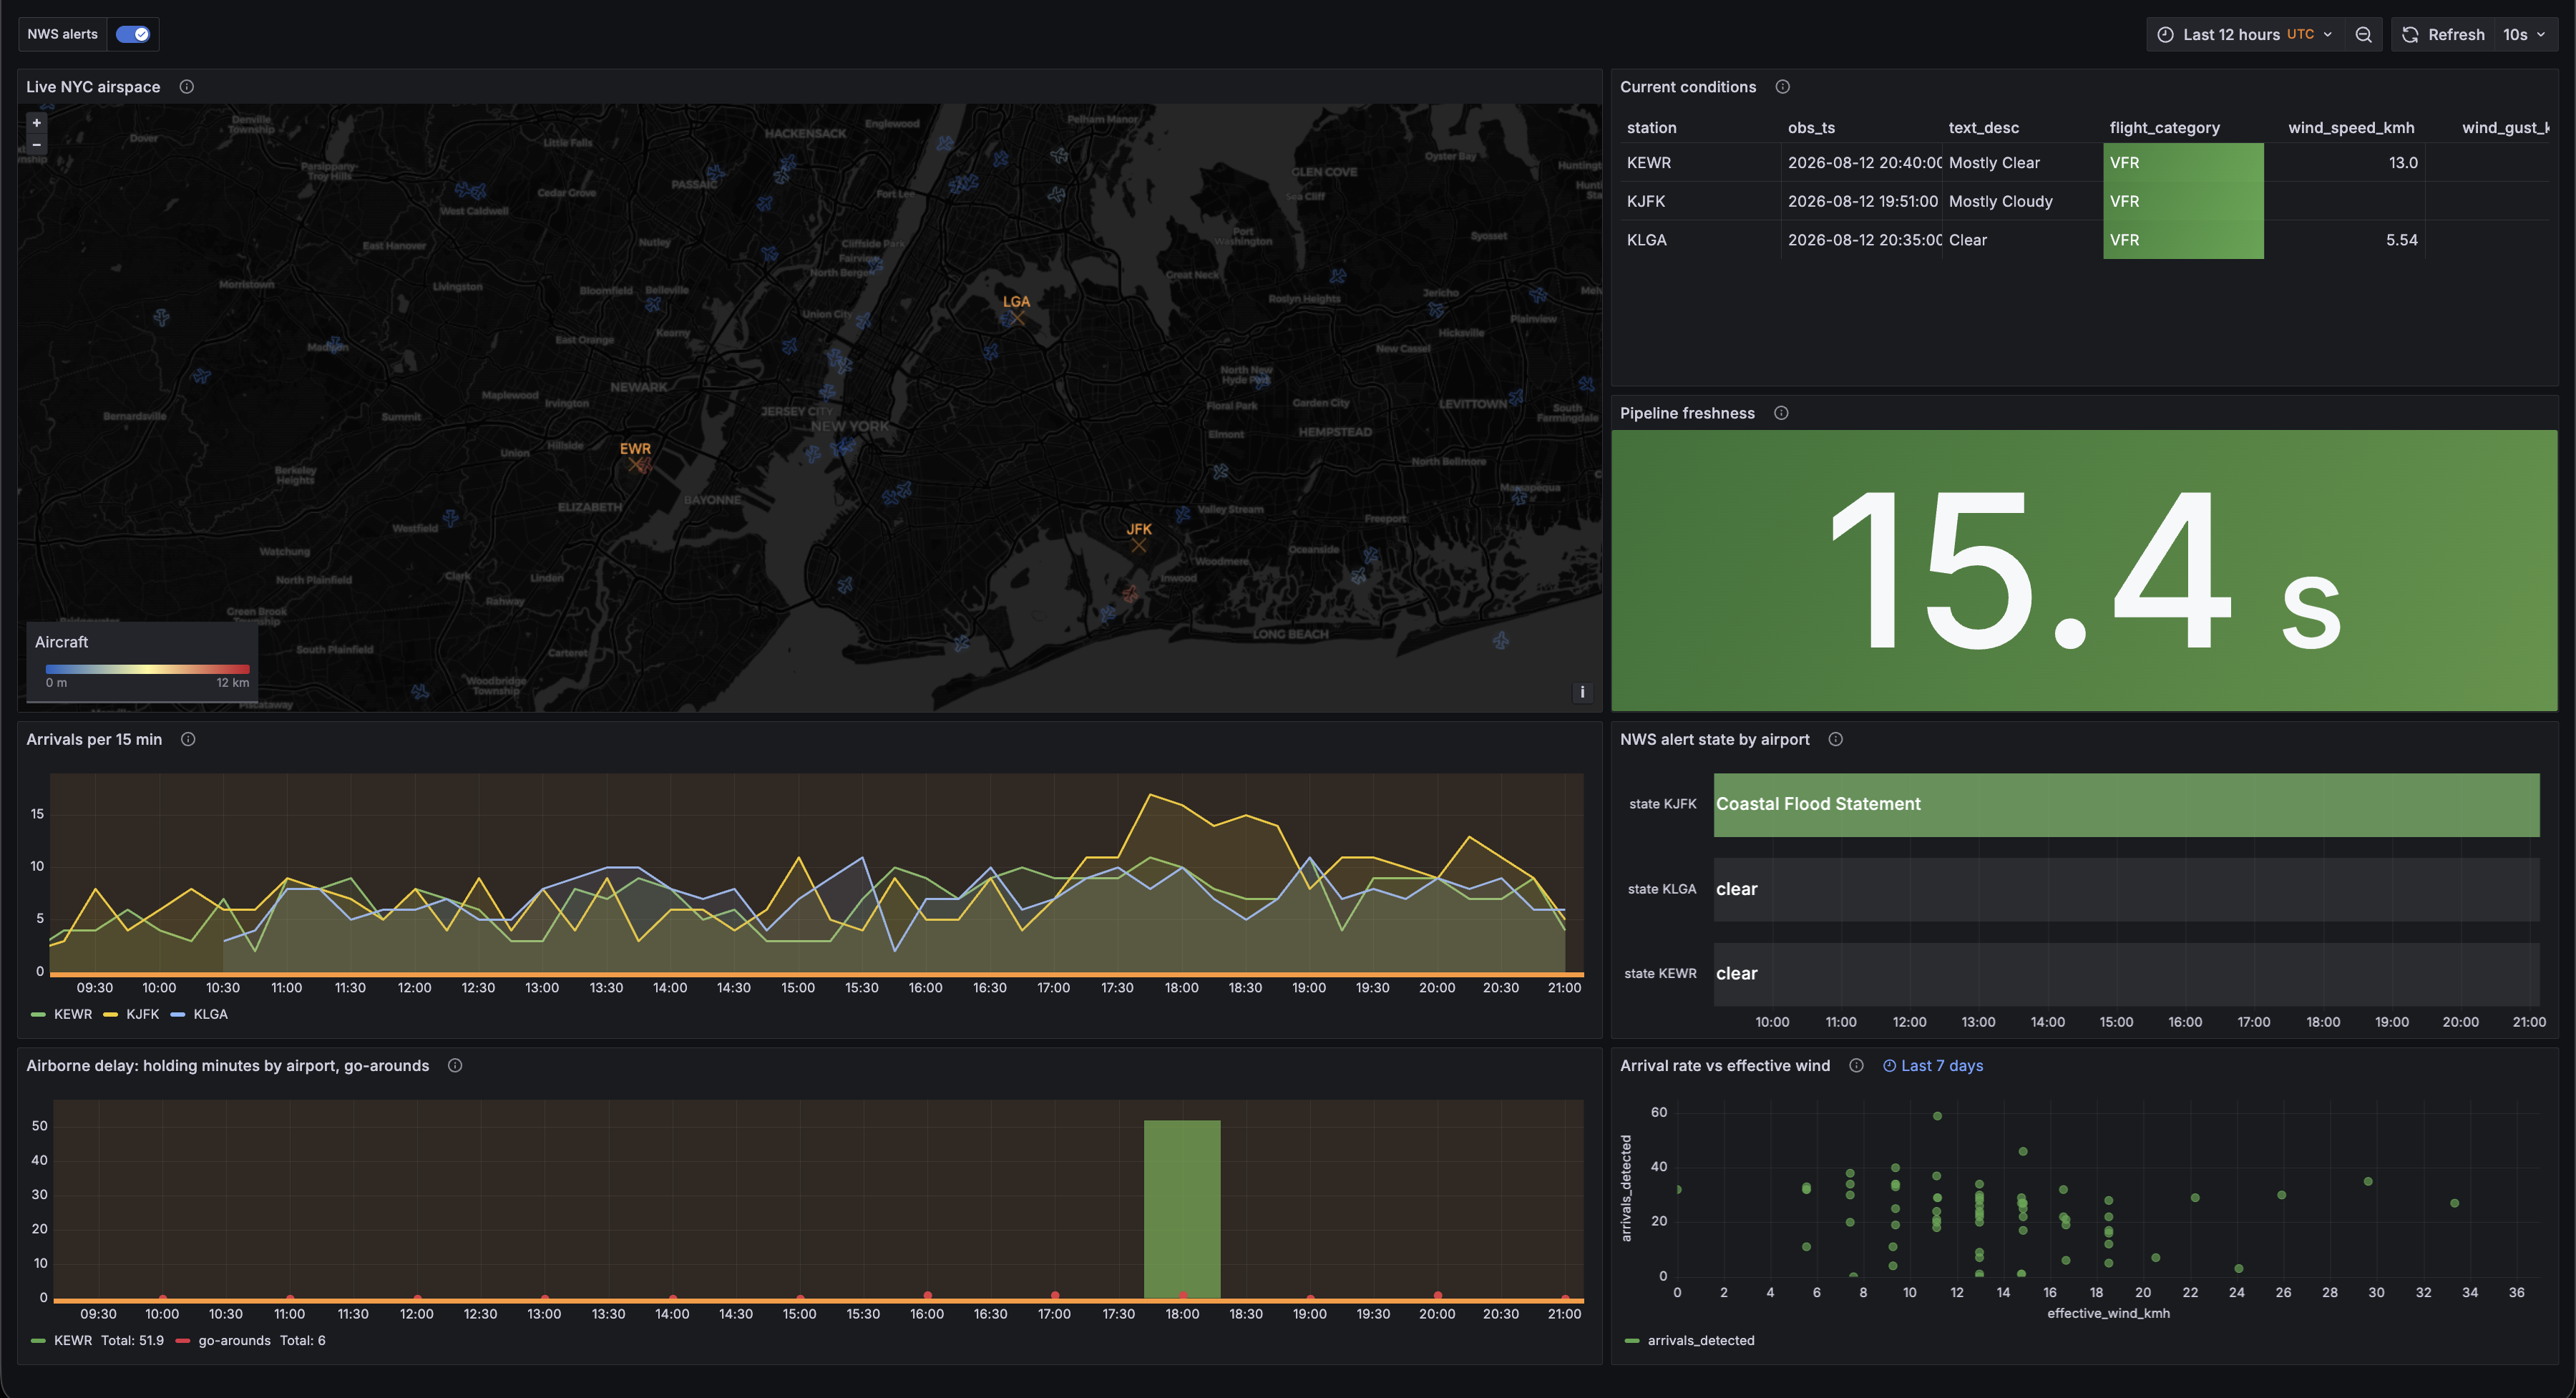
\includegraphics[width=\textwidth]{../assets/img/grafana-live-dashboard.png}
\caption{The live operations dashboard during the run: heading-rotated
aircraft colored by altitude, per-station flight category, pipeline freshness,
detected arrivals per 15 minutes with NWS alert windows overlaid.}
\end{figure}

Nine containers on one DigitalOcean droplet (8\,GB, Docker Compose): Kafka
(KRaft, single node), Postgres~16, Spark (single-node \code{local[*]},
three checkpointed streaming queries), two Python producers, a weather
consumer, Grafana, and the Dagster webserver and daemon. Azure held what must
survive the droplet: the immutable bronze archive and database backups.

Design decisions that carried the project:

\begin{itemize}
\item \textbf{Kafka at 5 messages per second} --- replay is the feature, not
throughput. The position API serves at most one hour of history, so the
retained log (7 days) is the only substrate detector tuning has. Both
production incidents were healed from it without data loss.
\item \textbf{Docker supervises streams; Dagster supervises batch.} An
orchestrator's run model is the wrong shape for an infinite process.
\item \textbf{Join-at-read, not stream-stream} --- weather is three
slowly-changing station records; events are enriched at query time with the
observation valid at event time.
\item \textbf{Units and nulls are load-bearing.} Every NWS quantity converts
by reading its \code{unitCode} (wind arrives in km/h); position-less
telemetry is counted and dropped, never interpolated; on-ground aircraft
legitimately report null altitude.
\item \textbf{Idempotency everywhere} --- deterministic event ids and upserts
on natural keys make replays and crash recovery unable to duplicate rows.
\end{itemize}

\section{Event detection}

Per-aircraft state machines over a ring buffer of recent position samples,
keyed by transponder address; Kafka partitioning guarantees per-aircraft
ordering into Spark's \code{applyInPandasWithState}.

\begin{itemize}
\item \textbf{Arrival} --- approach candidacy (near field, low, descending)
confirmed by ground contact, or by coverage loss on short final: transponder
contact commonly drops below ${\sim}450$\,m on approach, so a disappearance
there, confirmed by a 90-second state timeout, is an arrival.
\item \textbf{Holding} --- at least $340^{\circ}$ of cumulative unwrapped
track change within eight minutes without net displacement, inside the
holding altitude/speed band, filtered to airline-class traffic.
\item \textbf{Go-around} --- descent on approach followed by a committed
climb (two consecutive strong-climb samples, at least 200\,m regained) with
no touchdown.
\end{itemize}

Every threshold is a named constant. Tuning was done by replaying the
retained Kafka log with adjusted values and re-scoring against ground truth
--- never by eyeballing the map. The detectors have no Spark dependency; the
test suite runs the exact production logic over recorded live sequences,
including the captured poison sequence from the August~14 incident
(section~\ref{sec:ops}).

\section{Validation}

Every morning Dagster pulled the previous day's arrivals for the three
airports from OpenSky's independent arrivals record --- a source the
detectors never see --- and dbt scored each day per airport:
a detected arrival matches ground truth when the same airframe arrives at
the same airport within ten minutes. Precision is matched detected over all
detected; recall is matched ground truth over all ground truth.

The mart publishes both figures structurally, not on trust:

\begin{itemize}
\item Precision publishes only once the day's ground truth has landed at
plausible volume (at least half the detector's own count --- the upstream
aggregation can lag days).
\item Recall additionally requires the detection stream to have observed at
least 20 of 24 hours, measured stream-wide: an hour counts as observed when
any of the three fields recorded an arrival. A quiet overnight hour at one
airport is traffic, not coverage loss; a true outage silences all three
fields at once and still withholds the score.
\item An unscored day renders as a gap --- never as a zero. A partial day
and a bad day must never look alike.
\end{itemize}

\section{Results: the live run}

Fourteen days scored end to end (2026-08-12 through 2026-08-25; the first
partial day published precision only, and the final day of operation is
unscored because its ground truth publishes the following morning). Targets:
precision ${\geq}$\,85\%, recall ${\geq}$\,80\%, per airport per day.

\begin{table}[H]
\centering
\small
\begin{tabular}{lrrrrr}
\toprule
Airport & Scored days & Mean P & Min P & Mean R & Min R \\
\midrule
JFK      & 14 & 96.1\% & 89.4\% & 97.6\% & 92.8\% \\
LaGuardia & 14 & 97.8\% & 89.0\% & 95.8\% & 90.0\% \\
Newark   & 14 & 96.0\% & 87.0\% & 85.7\% & 76.3\% \\
\bottomrule
\end{tabular}
\caption{Detection quality over the full run (fully scored days). The single
target miss of the run is Newark's recall on August 24 (76.3\%), part of an
across-the-board dip that day --- every field's precision and recall fell
together, pointing at the day's data rather than any one detector. Every
other airport-day met both targets.}
\label{tab:live}
\end{table}

\begin{figure}[H]
\centering
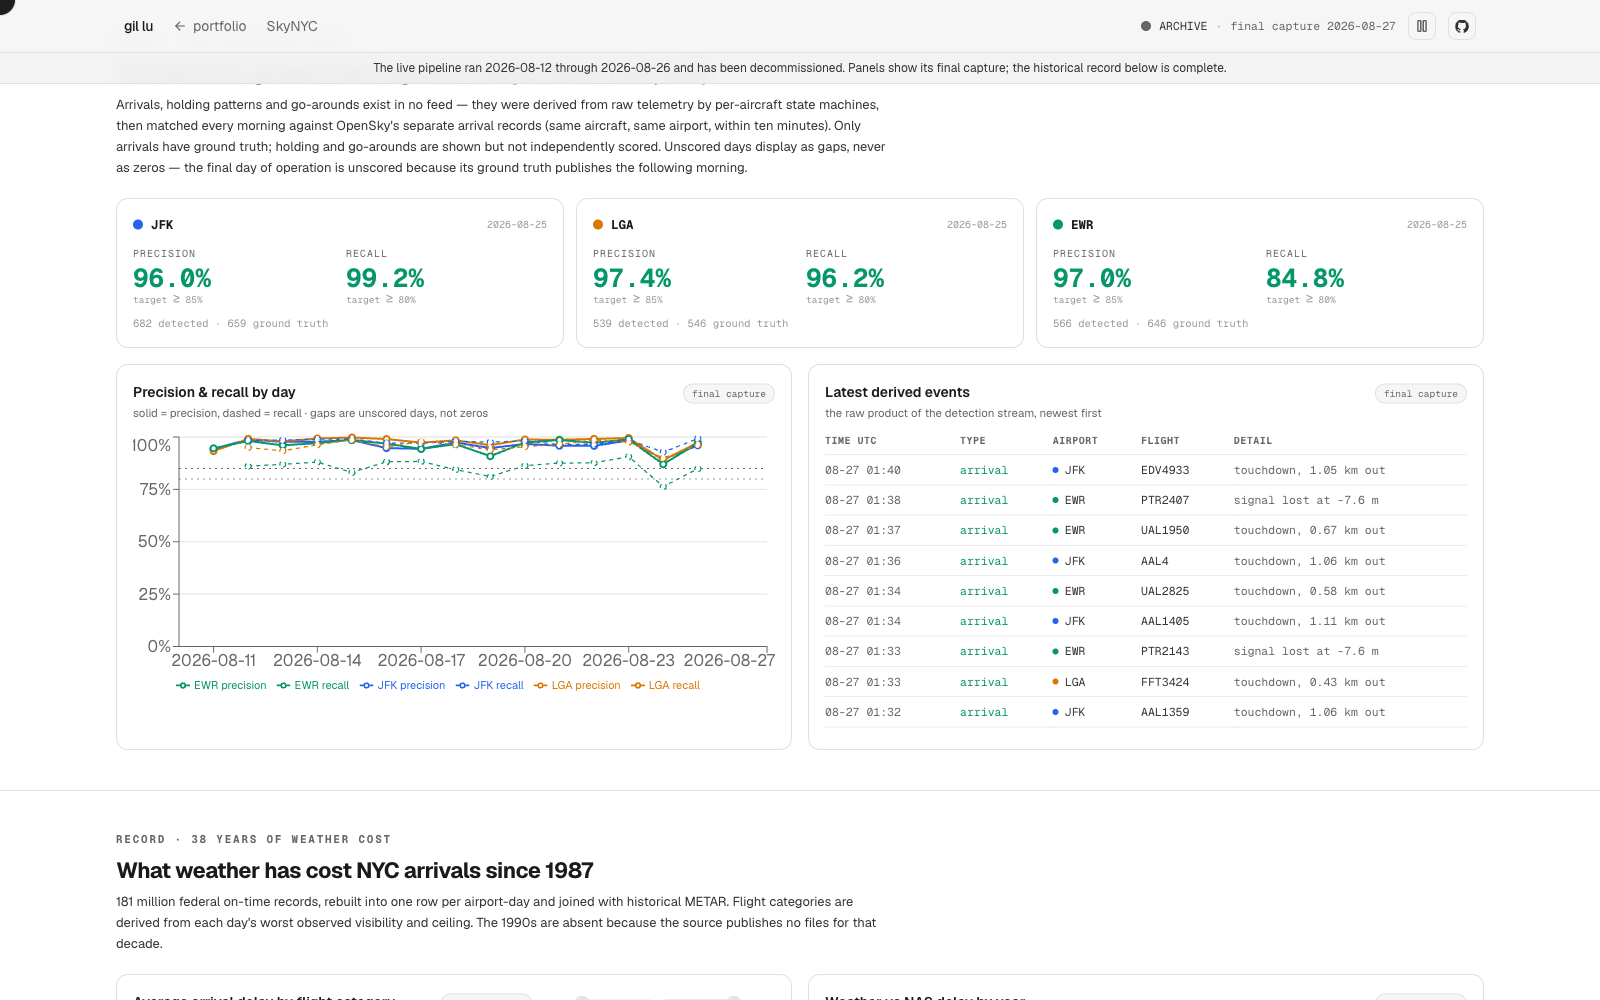
\includegraphics[width=\textwidth]{figures/web-proof.png}
\caption{The public dashboard's validation section at close: daily precision
(solid) and recall (dashed) per airport against the P${\geq}$85\% /
R${\geq}$80\% targets, and the final scored day's tiles.}
\end{figure}

\subsection{Weather during the run}

The run was mostly benign August VFR, which is exactly what makes its two
severe episodes legible in the event stream.

\textbf{August 20 --- evening convective flooding.} The National Weather
Service issued Severe-severity Flash Flood Warnings covering all three
fields from 21:39\,UTC to 00:15\,UTC (with a Special Marine Warning over the
JFK approaches and a Flood Watch that stayed in effect into the following
week). The stations recorded the worst conditions of the run: LaGuardia
dropped to LIFR at 805\,m visibility with a 41.9\,mm/hr rain rate, and
Newark gusted to 78\,km/h. The operational response is visible hour by
hour: the arrival rate across the three fields fell from 103/hr at 18:00 to
27/hr at 22:00 --- a 74\% collapse --- and the recovery push at
02:00--03:00\,UTC carries the day's concentration of holding patterns and
go-arounds. Ground truth dipped the same way (1{,}542 recorded arrivals
against a ${\sim}$1{,}800 typical day: cancellations and diversions, not
detector loss), and the day scored normally --- precision 96.7--98.8\%.

\textbf{August 23 --- morning flash flooding.} A second episode brought
Flash Flood Warnings to the fields from 10:12 to 13:15\,UTC, with rain
rates to 24\,mm/hr and IFR visibility. The operational effect was milder
(1{,}607 arrivals, a modest dip); the day scored 98.3--99.5\% precision.

\textbf{August 17 --- IFR morning.} The run's third-worst day was not a
storm but low ceilings: 116 IFR/LIFR observations across the stations, and
the run's second-highest holding count (24 events).

\begin{table}[H]
\centering
\small
\begin{tabular}{lllrrr}
\toprule
Date & Worst alert in effect & Worst obs. & Arrivals & Holding & Go-arounds \\
\midrule
08-17 & --- & IFR, 2.8\,km vis & 1{,}817 & 24 & 5 \\
08-20 & Flash Flood Warning (Severe) & LIFR, 805\,m vis, 78\,km/h gust & 1{,}479 & 9 & 7 \\
08-23 & Flash Flood Warning (Severe) & IFR, 24\,mm/hr rain & 1{,}607 & 2 & 2 \\
\bottomrule
\end{tabular}
\caption{The run's turbulent-weather days against a ${\sim}$1{,}800-arrival
typical day. August 20 is the run's clearest demonstration of the thesis:
severe weather arrived, the arrival rate collapsed within the hour, and the
detectors kept scoring through it.}
\label{tab:weather}
\end{table}

\begin{figure}[H]
\centering
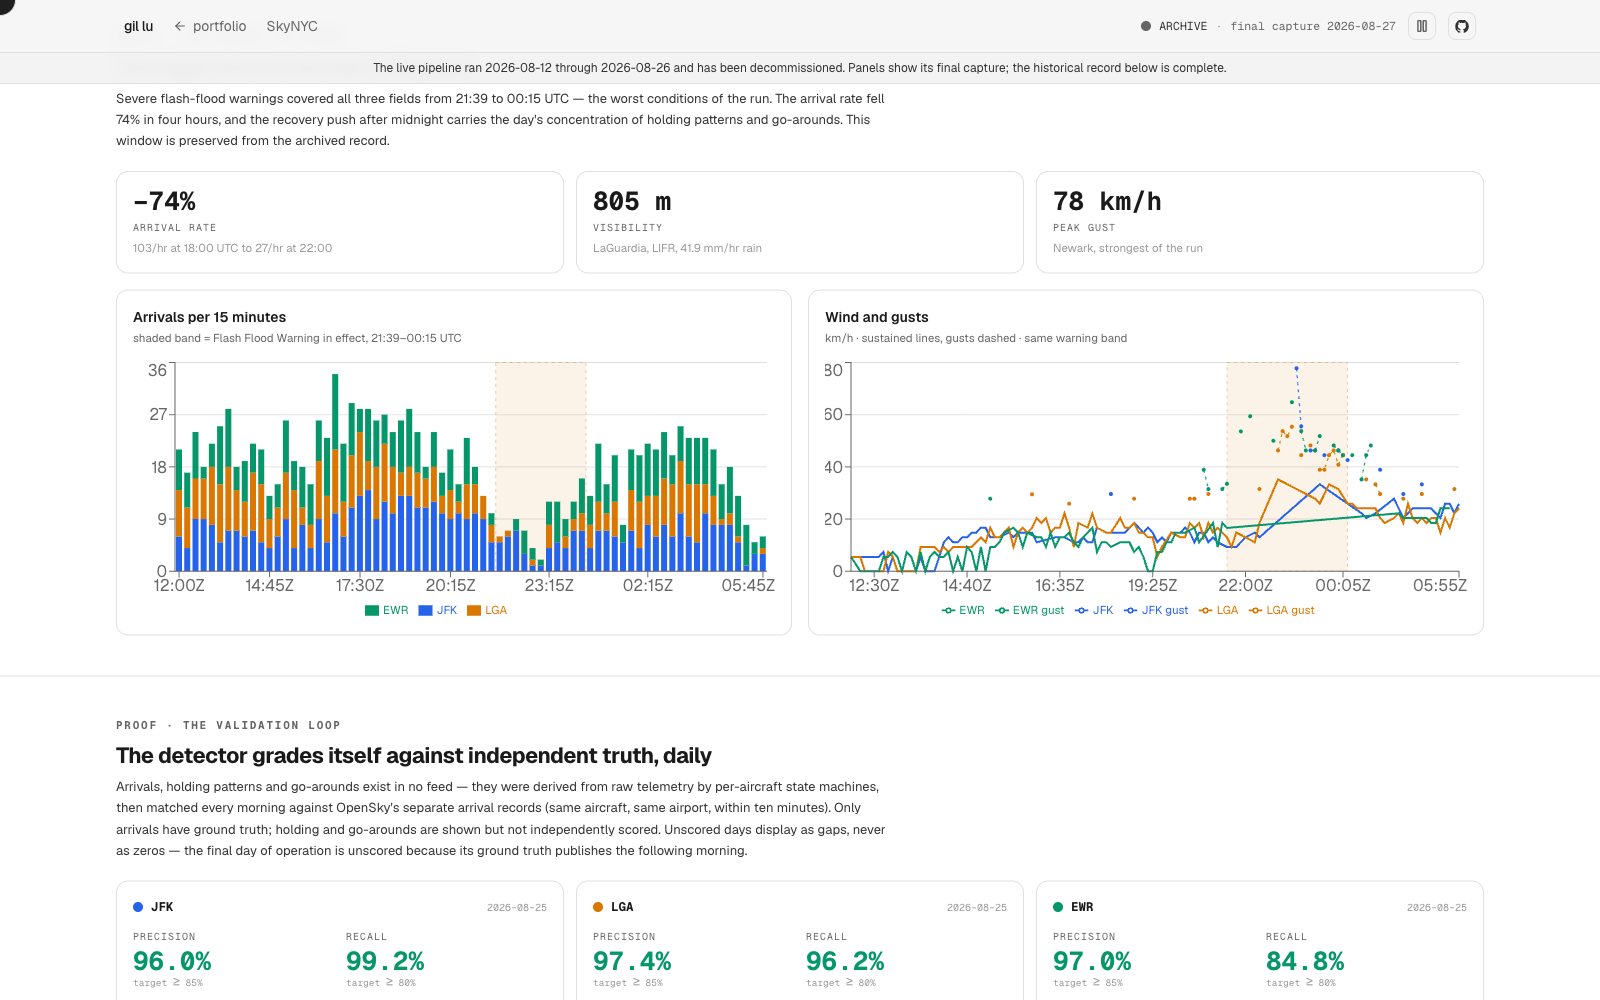
\includegraphics[width=\textwidth]{figures/web-storm.png}
\caption{The storm as the public dashboard now presents it: the collapse
and recovery in 15-minute arrival bars, wind and gusts across the three
stations, and the Flash Flood Warning interval shaded on both charts. The
window ships with the page as a static slice of the archived record.}
\end{figure}

\begin{figure}[H]
\centering
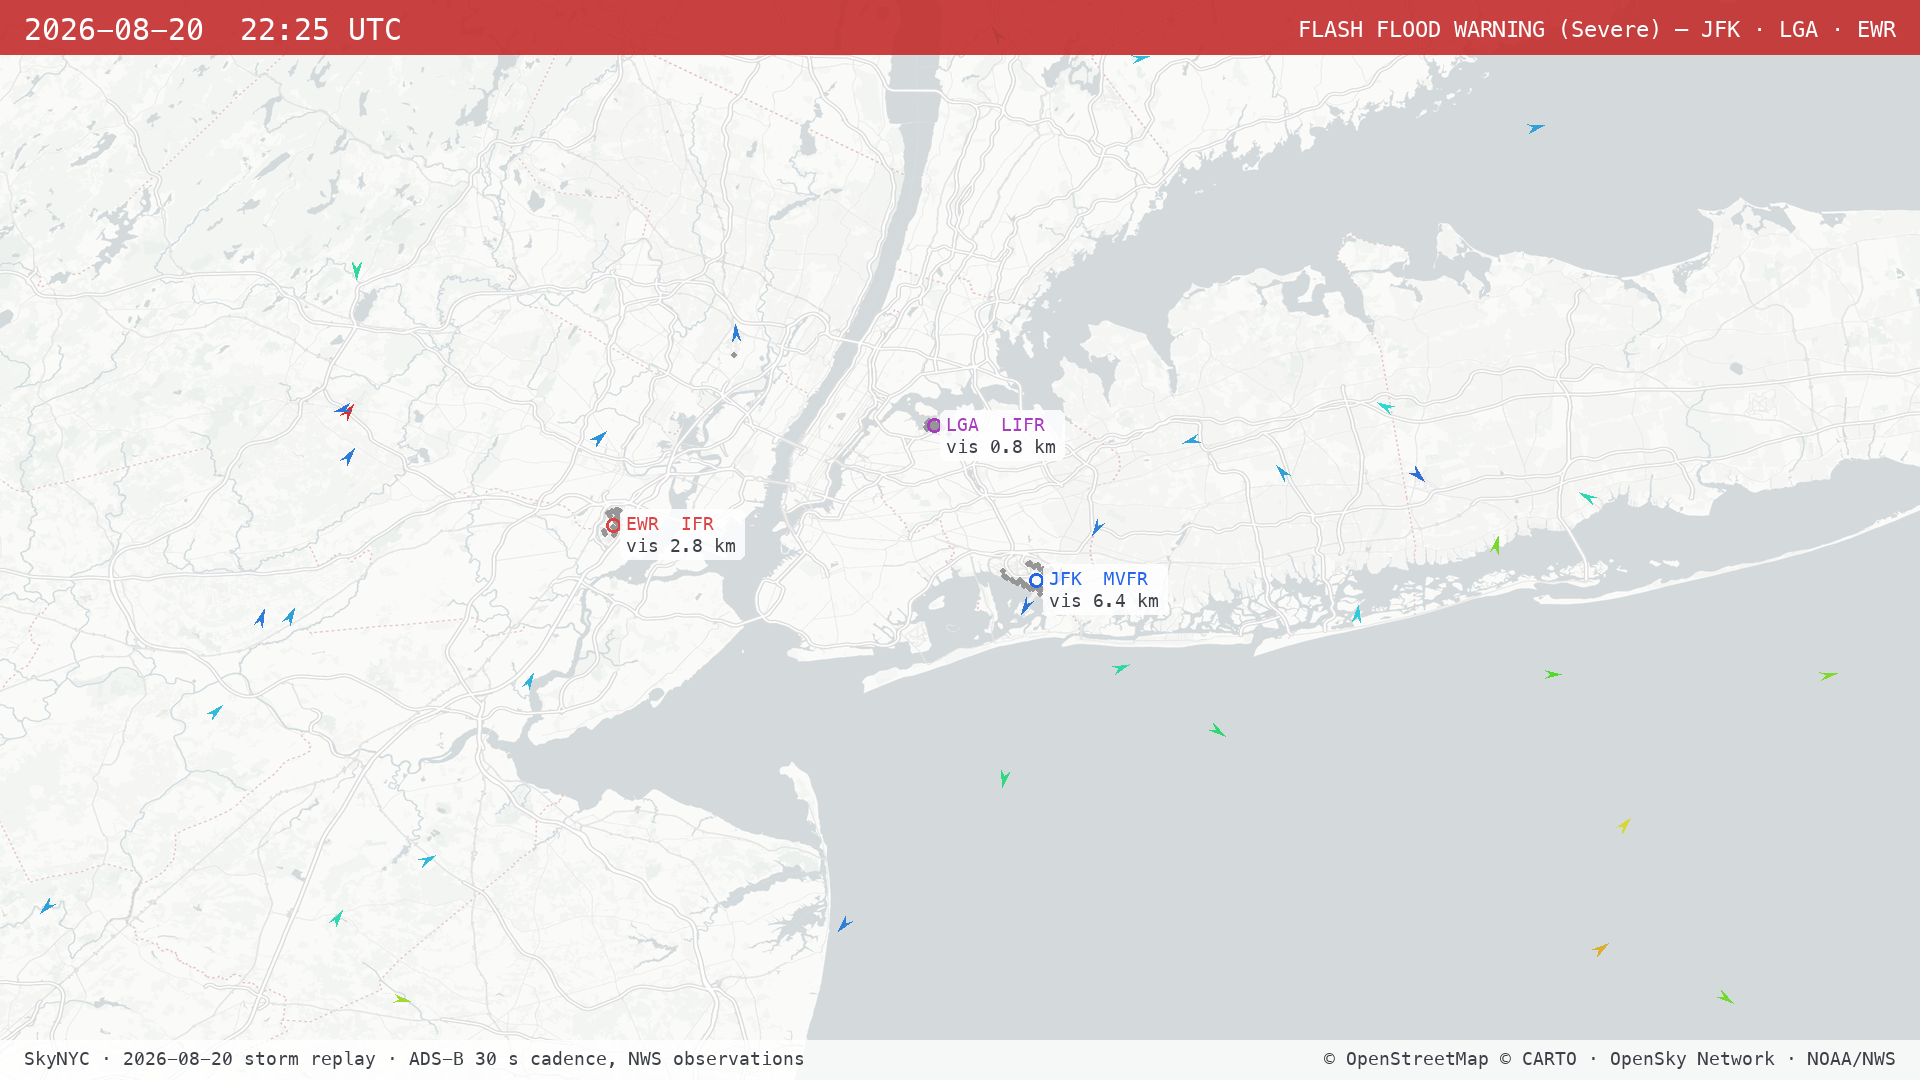
\includegraphics[width=\textwidth]{figures/storm-replay-frame.png}
\caption{A frame from the storm replay at 22:25\,UTC --- the trough of the
collapse. Aircraft positions from the archived bronze telemetry (colored
by altitude), station chips carrying the observation valid at frame time:
LaGuardia LIFR at 0.8\,km visibility, Newark IFR, the warning banner
active. The full 48-second replay of the six-hour window accompanies the
repository at \code{assets/video/storm-replay-2026-08-20.mp4}.}
\end{figure}

One capture caveat: alerts were stored for the three airport points only,
so a warning polygon elsewhere in the metro area --- a tornado warning
included --- would not appear in this record unless it covered a field.

\subsection{Newark's recall}

Newark's recall ran consistently below the other two fields
(76.3--90.6\%, mean 85.7\%). The pattern is structural, not noise: EWR sits at the
edge of the receiver coverage the detectors work from, and its
arrival flows more often descend below reliable coverage earlier in the
approach, so more true arrivals produce too few samples to confirm. The
precision guard means what the detector does claim at Newark is still right
--- the miss cost lands on recall alone, which is the honest side to pay it.

\section{Results: 38 years of weather cost}

The historical medallion quantifies the thesis at climatological scale.
Table~\ref{tab:thesis} aggregates 31{,}413 airport-days (1987--2026; BTS
publishes no files for 1990--1999) by each day's worst observed flight
category.

\begin{table}[H]
\centering
\small
\begin{tabular}{llrrr}
\toprule
Airport & Category & Avg.\ arrival delay (min) & Cancelled & Days \\
\midrule
JFK & VFR  &  2.0 & 1.2\% & 5{,}428 \\
    & MVFR &  7.5 & 2.1\% & 1{,}835 \\
    & IFR  & 16.1 & 3.5\% & 1{,}537 \\
    & LIFR & 22.9 & 5.5\% & 1{,}669 \\
\midrule
LGA & VFR  &  2.1 & 2.1\% & 5{,}428 \\
    & MVFR &  7.8 & 3.2\% & 1{,}952 \\
    & IFR  & 17.6 & 5.3\% & 1{,}686 \\
    & LIFR & 29.7 & 9.7\% & 1{,}403 \\
\midrule
EWR & VFR  &  4.1 & 1.6\% & 5{,}305 \\
    & MVFR & 10.7 & 2.6\% & 1{,}962 \\
    & IFR  & 21.9 & 4.7\% & 1{,}800 \\
    & LIFR & 31.1 & 8.1\% & 1{,}402 \\
\bottomrule
\end{tabular}
\caption{Average arrival delay and cancellation rate by the day's worst
observed flight category, 1987--2026. Delay climbs monotonically at every
airport --- roughly $11\times$ VFR-to-LIFR at JFK, $14\times$ at LaGuardia,
$8\times$ at Newark --- and cancellation rates climb four- to five-fold.}
\label{tab:thesis}
\end{table}

\begin{figure}[H]
\centering
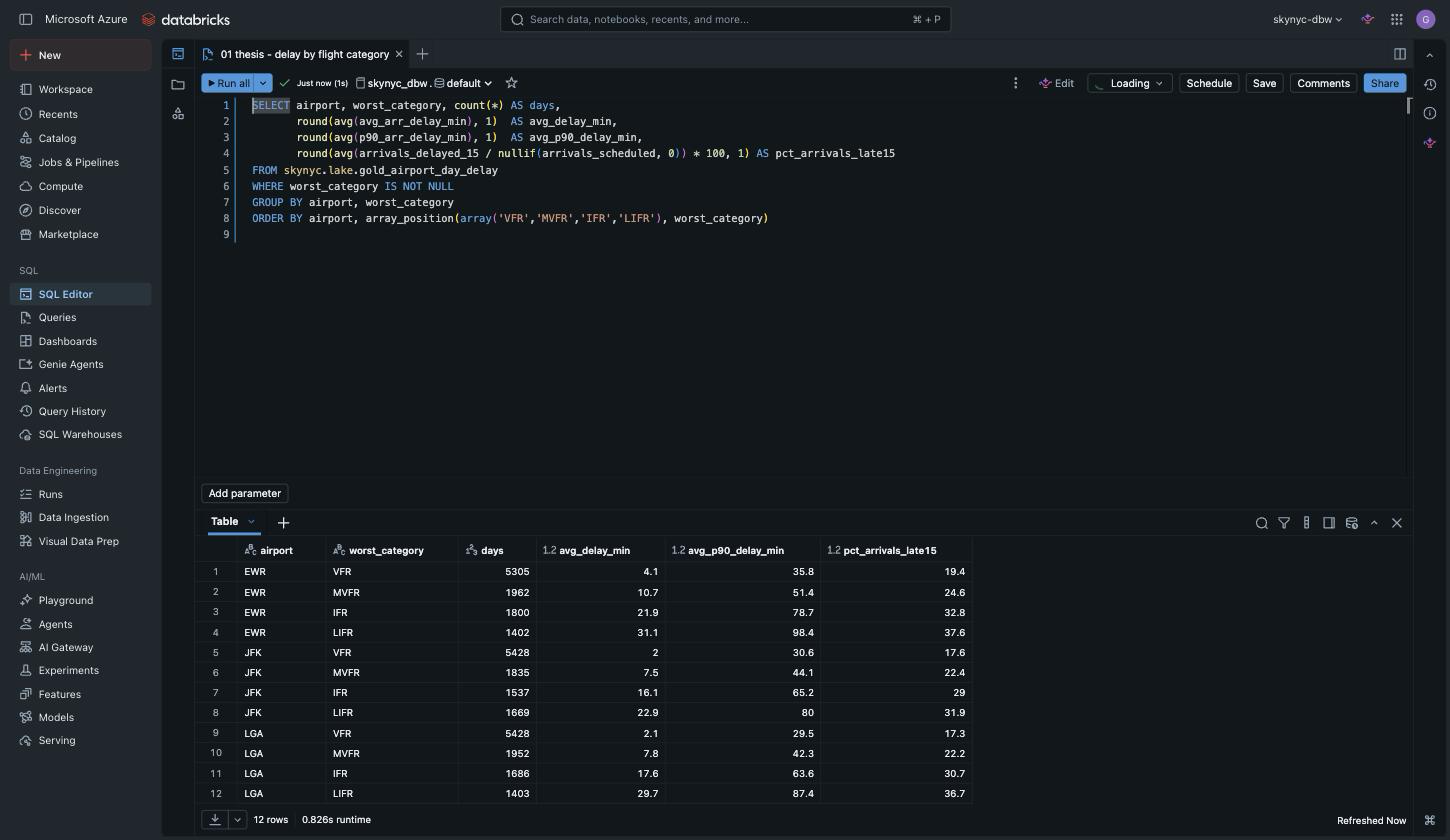
\includegraphics[width=\textwidth]{../assets/img/databricks-sql-thesis.png}
\caption{The thesis in one query on the serverless warehouse over the gold
Delta tables, sub-second: arrival delay by flight category across the full
record.}
\end{figure}

Visibility and ceiling --- the components of flight category --- are the
strongest leading indicators in the record; wind and gusts matter most
through runway-configuration changes, which show up as IFR-day delay
variance rather than as an independent monotonic effect.

\section{Operations}
\label{sec:ops}

The live layer ran continuously from 2026-08-12 to 2026-08-26 on one
droplet. Steady state: about 4.7\,GB RAM across nine containers, three
streaming queries each completing micro-batches well inside their trigger
intervals, and the upstream API quota never exhausted. Two incidents
occurred; both were diagnosed from evidence, fixed at the root, and healed
without data loss.

\subsection{Incident 1: NaN poisoning (Aug 14--15)}

The events streaming query entered a crash loop: pandas represents nullable
doubles as \code{NaN}, which passes \code{is None} guards, compares false
against every threshold, and survives \code{json.dumps} as a literal
\code{NaN} that Postgres's \code{jsonb} rejects. One poisoned record made
the micro-batch fail and replay from the checkpoint --- 1{,}600+ restarts
over 23 hours. The fix normalized \code{NaN} to \code{None} at both seams
where the Spark bridge hands the detectors data: the message boundary and
the decoded state blob (state written before the first fix retained the
poison, which is why fixing only the message boundary did not recover the
stream). The gap was replayed in full from the retained Kafka log; the
poison sequence was captured into the test suite. Producers and the live
path never went down.

\subsection{Incident 2: silent scheduler stop (Aug 23)}

Dagster's scheduler daemon thread hung at 19:00~UTC evaluating an hourly
schedule --- no exception, no restart, container healthy, every other
daemon thread still heart-beating. Scheduled work simply stopped: no more
hourly builds, ground-truth pulls, or quality scoring. Detection itself was
unaffected (streams are supervised by Docker, not Dagster --- the
separation held exactly as designed). The stop was diagnosed from the
per-daemon heartbeat table; restarting the daemon let the scheduler's
catch-up fire the missed ground-truth partitions, and the idempotent
upsert-everywhere design meant three days of scores backfilled cleanly with
no special handling. Lesson recorded: container-level health checks do not
see thread-level death; liveness monitoring must watch the heartbeat the
component itself emits.

\section{Cost and resource footprint}

\begin{table}[H]
\centering
\small
\begin{tabular}{lrl}
\toprule
Item & Cost & Notes \\
\midrule
DigitalOcean droplet & \$26 & 4\,GB tier resized in place to 8\,GB; hourly \\
 & & billing, 2026-08-11 to 2026-08-27, destroyed at close \\
Azure (ADLS, ADF, Databricks) & ${\sim}$\$10--15 & most of it the one-time medallion build \\
Vercel (frontend + blob) & \$0 & free tier; hosts the permanent archive \\
\midrule
Total & \textbf{${\sim}$\$36--41} & \\
\bottomrule
\end{tabular}
\caption{Infrastructure cost, complete.}
\end{table}

The allocation behind those numbers ran deliberately close to the metal:

\begin{itemize}
\item \textbf{One 8\,GB / 4-vCPU droplet} carried all nine containers at a
steady ${\sim}$4.7\,GB RAM --- the Spark driver (4\,GB heap) owning half,
Kafka and Postgres most of the rest. CPU load averaged well under half the
box. Resizing from the 4\,GB tier the day the Spark driver deployed cost
about a minute of downtime; the restart policies brought the stack back
unaided.
\item \textbf{Storage at close:} the streaming bronze archive measured
1.5\,GB across 175{,}801 Parquet objects; the historical layer's raw
landing zone 9.0\,GB and its Delta medallion 14.3\,GB; the entire serving
database compressed to a 14\,MB dump. Disk on the droplet --- Kafka's
7-day retained log included --- peaked at 22\,GB of the 154 available.
\item \textbf{Batch compute} was single-node by construction: bronze
ingestion is per-archive (ZIPs are not splittable), so the 181M-row
medallion build ran on one auto-terminating Databricks node in
${\sim}$3.5 hours end to end, and worker count remains a single Terraform
variable where the workload to justify it appears.
\item \textbf{API quota as a resource:} the position poll spent 1 credit
per 30\,s call (${\sim}$2{,}880/day of the 4{,}000 allowance) with a
degrade-cadence guard; the ground-truth pull cost 36/day from a separate
bucket. Neither was ever exhausted.
\end{itemize}

\section{Decommissioning}

The project concluded 2026-08-26. Compute was destroyed; everything durable
was preserved first:

\begin{itemize}
\item Final ground-truth pull, quality scoring, and mart build completed,
so the record closes on a fully scored day (2026-08-25).
\item Final \code{pg\_dump} archived locally and off the droplet.
\item The public dashboard (\href{https://sky.gillu.me}{sky.gillu.me})
now serves its final capture from static storage --- the page states it is
an archive, the map shows the final positions, and the historical sections
remain complete. Outliving its own pipeline was a designed property, not an
afterthought.
\item The droplet and the Azure resource group (lake, Data Factory,
Databricks workspace) were deleted; no billable resources remain.
\end{itemize}

\begin{figure}[H]
\centering
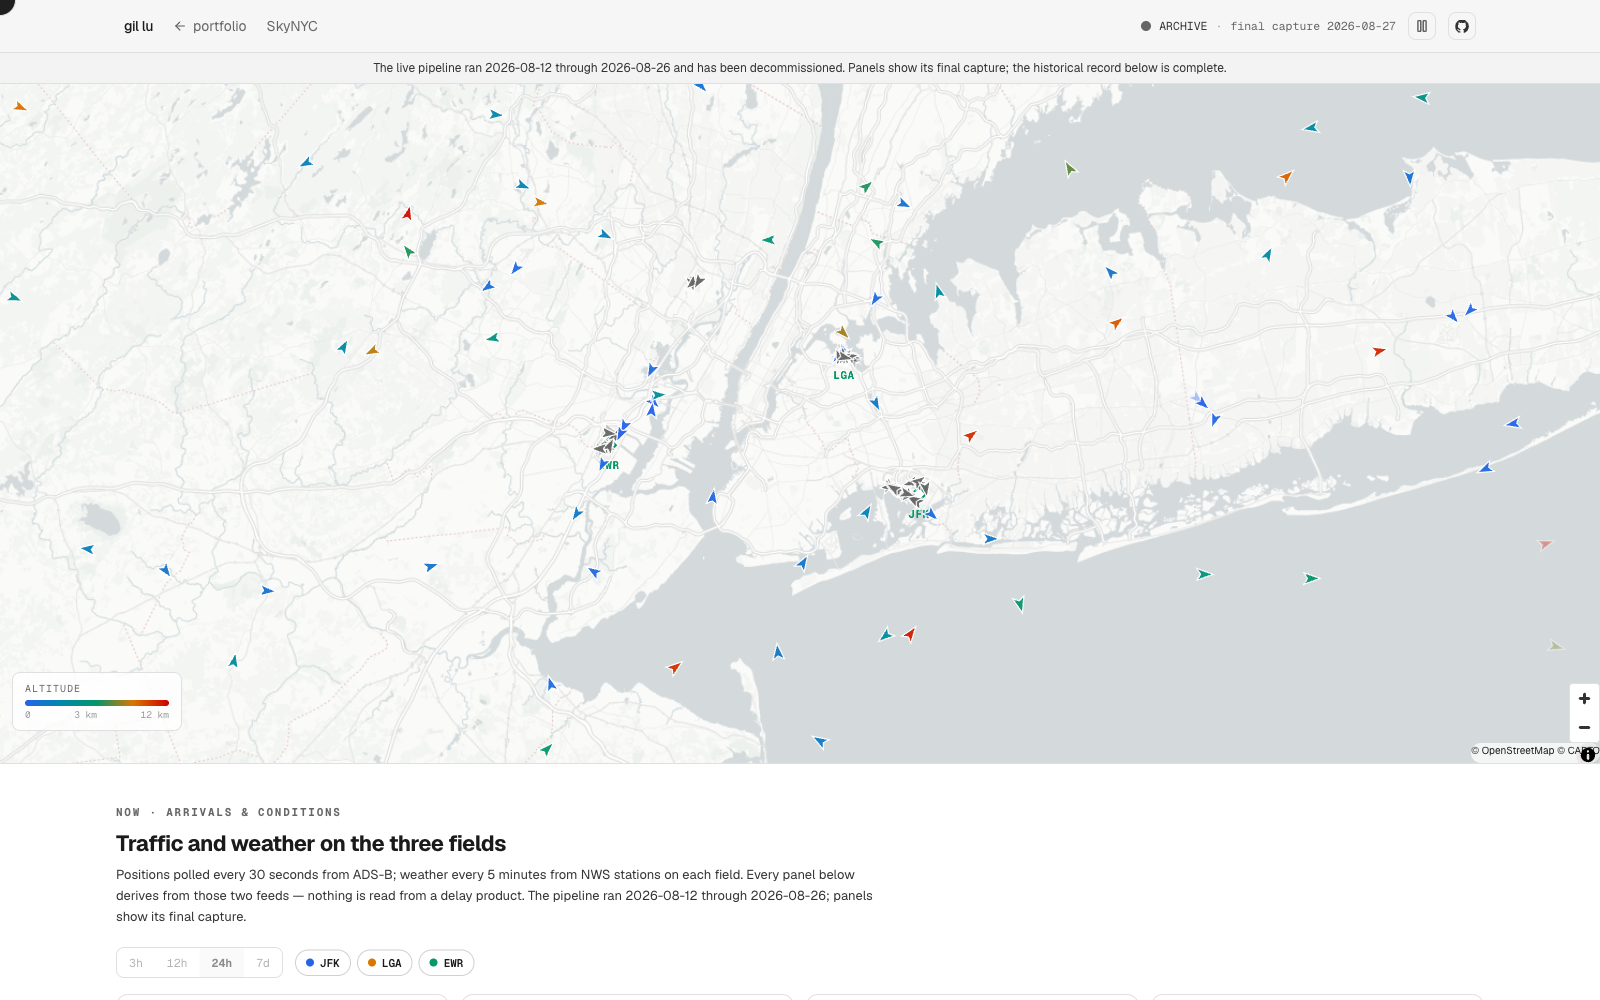
\includegraphics[width=\textwidth]{figures/web-archive.png}
\caption{The public dashboard in its final state: the archive banner, the
final captured positions, and per-field conditions at close.}
\end{figure}

\section*{Data sources}

\begin{itemize}
\item \textbf{OpenSky Network} --- aircraft state vectors and arrival
records, research/non-commercial terms. M.~Schäfer, M.~Strohmeier,
V.~Lenders, I.~Martinovic, M.~Wilhelm. \emph{Bringing Up OpenSky: A
Large-scale ADS-B Sensor Network for Research}. IPSN 2014.
\item \textbf{NOAA / National Weather Service} --- station observations and
active alerts, US-government open data.
\item \textbf{U.S. BTS TranStats} --- on-time performance, 1987--2026.
\item \textbf{Iowa Environmental Mesonet} --- historical METAR.
\end{itemize}

\appendix
\section{Daily scores}

Percent, as published by \code{mart\_detection\_quality}. A dash is a
withheld score, not a zero: August 11 was a partial first day (five observed
hours), so recall is withheld; August 10 predates detection entirely; August
26's ground truth publishes after decommissioning.

\begin{table}[H]
\centering
\small
\begin{tabular}{lrrrrrr}
\toprule
 & \multicolumn{2}{c}{JFK} & \multicolumn{2}{c}{LaGuardia} & \multicolumn{2}{c}{Newark} \\
Date (2026) & P & R & P & R & P & R \\
\midrule
08-11 & 94.4 & --- & 93.3 & --- & 94.6 & --- \\
08-12 & 98.8 & 98.5 & 99.1 & 95.0 & 98.1 & 86.1 \\
08-13 & 97.7 & 98.6 & 98.0 & 93.4 & 96.0 & 87.0 \\
08-14 & 97.8 & 98.9 & 99.3 & 96.3 & 97.1 & 88.0 \\
08-15 & 98.5 & 99.1 & 99.8 & 98.6 & 98.6 & 83.1 \\
08-16 & 94.7 & 97.1 & 99.0 & 95.3 & 96.8 & 88.2 \\
08-17 & 94.4 & 97.0 & 97.3 & 97.9 & 94.3 & 88.3 \\
08-18 & 97.4 & 97.9 & 98.4 & 96.3 & 96.6 & 84.4 \\
08-19 & 94.7 & 97.6 & 96.1 & 93.9 & 90.8 & 81.1 \\
08-20 & 96.7 & 98.2 & 98.8 & 95.4 & 97.4 & 86.3 \\
08-21 & 95.8 & 96.4 & 98.7 & 96.5 & 98.6 & 87.6 \\
08-22 & 95.8 & 96.7 & 99.1 & 98.6 & 97.3 & 87.7 \\
08-23 & 98.3 & 98.6 & 99.5 & 97.5 & 98.8 & 90.6 \\
08-24 & 89.4 & 92.8 & 89.0 & 90.0 & 87.0 & 76.3 \\
08-25 & 96.0 & 99.2 & 97.4 & 96.2 & 97.0 & 84.8 \\
\bottomrule
\end{tabular}
\caption{Daily precision and recall per airport, full run.}
\end{table}

\end{document}
